\section{Methods}
This section will explain the overall architectural pipeline that will be used in 
order to implement the required models and agents to perform the following behavior,
which is illustrated in Figure \ref{pipeline}. This pipeline will be implemented 
in two phases: an offline and online phase. Both of these will be discussed. 
Finally the hardware used in this thesis will be explained.

\begin{Figure}
    \centering
    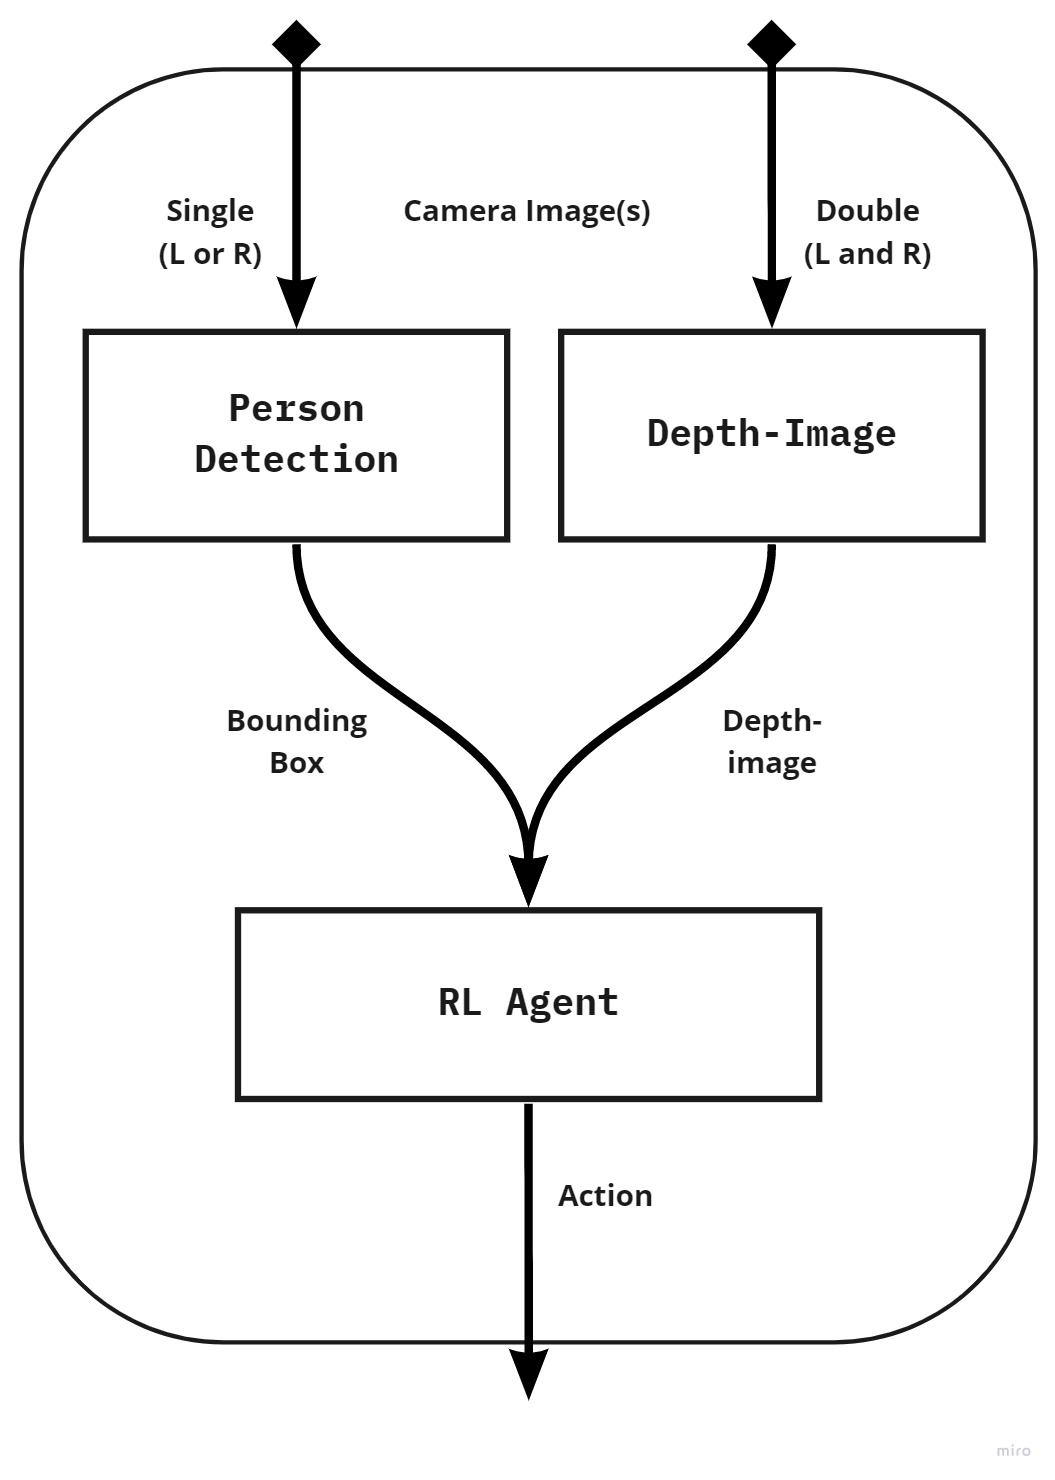
\includegraphics[width=\linewidth]{Pipeline.jpg}
    \captionof{figure}{The pipeline to be implemented}
    \label{pipeline}
\end{Figure}

\subsection{Goal}
The desired behavior for the drone is to follow the person. For this thesis, 
this can be interpreted in a wide sense of the word: as long as the person 
is in the center vision of the camera of the drone, this task is being
fulfilled. Translated to the inputs that the drone will receive, this 
means that the drone should maintain a bounding box as much 
in the center of its image input as possible. This can easily be 
calculated by simply taking the middle of the bounding box produced by the 
object detector. Bringing this point as close as possible to the center 
point of its image, is what the RL agent would need to learn. Next to 
defining the problem statement, this simultaneously 
removes the need to specify what distance the drone would need to fly from 
because the system can decide on its own what the perfect angle and distance 
will be to perform this task. 

\subsection{Pipeline}
To perform this succesfully, the pipeline, as illustrated in Figure \ref{pipeline}, 
will be implemented. This pipeline includes an object detector, 
depth-perception technology and a RL agent, each of which will be discussed 
further.

\subsubsection{Object Detection}
Longduring efforts to reduce the 
computational weight of object detection models has resulted in a set of networks 
that can operate in some capacity on the RP \cite{yolov3-tiny,Mixed-Yolo_Lite,YOLO-Lite}. 
However, 
since the rest of the pipeline also needs to be implemented on the RP, the need for the 
lightest of these models is required in this thesis. For this reason, YOLO-Fastest \cite{YOLO-Lite} 
will be used. This model only takes up a total of 1.3MB in size and has a 4.4ms 
runtime, which is the fastest of the slimmed YOLO versions. The reported mAP on the 
VOC dataset is 23.65\% for the smallest version. 
The latest YOLOv4 \cite{YOLOv4} 
has a mAP of over 43.5\% on the VOC dataset. This does not compare directly, 
but this does give a good indication for the possible results.  

Since the models are built to distinguish a multitude of classes and this thesis 
only requires one class, a person, the model would need slight fine-tuning. This 
can be done by performing transfer learning. By freezing all the layers except 
for the last classification layer, and retraining this layer, the desired class 
detection will be achieved. This process will result in a smaller network leading to 
faster inference, while not losing in performance. 

\subsubsection{Depth-Perception}
The next aspect of the pipeline will be the depth-perception. Since this thesis 
consists of two stages, an offline and online phase, there is a distinction 
in how the depth-imaging is performed. In the offline phase, which will take 
place in a simulated environment, the depth-image is being provided by the 
simulation itself. Since this simulation has full access to the ground truth, an 
accurate depth-view can be produced. However, during the online phase, this is not 
the case. Here the choice of technology has been to implement stereo vision. 
This means that there will be two images from two cameras, resulting in a left and right image.
These two images will have to be processed into a depth-image which
will be performed using the OpenCV library, a library which is 
specialized in performing computer vision operations. This will produce a depth-image 
with a slight margin of error, however. Whether the trained network in the 
offline phase can generalize to the real-world will be investigated 
in the online phase. 

\subsubsection{Reinforcement Learning Agent}
After object detection, the next aspect is to implement an RL agent for the use 
of determining what actions to take in each situation. The training stage of 
this agent will happen using a virtual environment. The ability to command a 
drone in a virtual environment will be used to model the situation as it would 
be on the physical drone. This simulation drone will receive the same camera inputs 
as the physical drone, which will be an image of the camera on the drone and a 
corresponding depth image. The normal image will be used for performing the object 
detection. The depth-image will be used as an input for the RL agent, together 
with the bounding box.

\subsection{Offline Phase}
The deployment of the pipeline will happen in two stages. The first stage, the offline 
stage, will be training the RL agent in a virtual environment. In order to do this, 
the full pipeline must be implemented in a simulation. This section will elaborate 
on the choice of simulation program, environments used for training and delineate the 
training process. 

\subsubsection{Simulation Program}
The program used to implement and train the agent will be Microsoft's  
AirSim \cite{airsim}. Based on the Unreal Engine \cite{unrealengine}, 
the simulation allows for a multitude of created environments to be used. Next 
to this, the program allows the user to instantiate a quadcopter directly in a 
virtual environment, together with simulated vision possibilities including a 
normal camera and depth-view, making this the preferred option. These views can 
be observed at the bottom of Figure \ref{airsim}. Additionally, the ability to 
command the vehicles through a Python or C++ script, makes AirSim very suitable 
to perform Deep Learning. What makes it even more attractive, is that AirSim allows 
easy connectivity with the PixHaw API, which, as will be explained later, is also 
used to control the physical drone. Once the agent has been trained, this makes 
the transfer to the physical drone much easier. 

\begin{Figure}
    \centering
    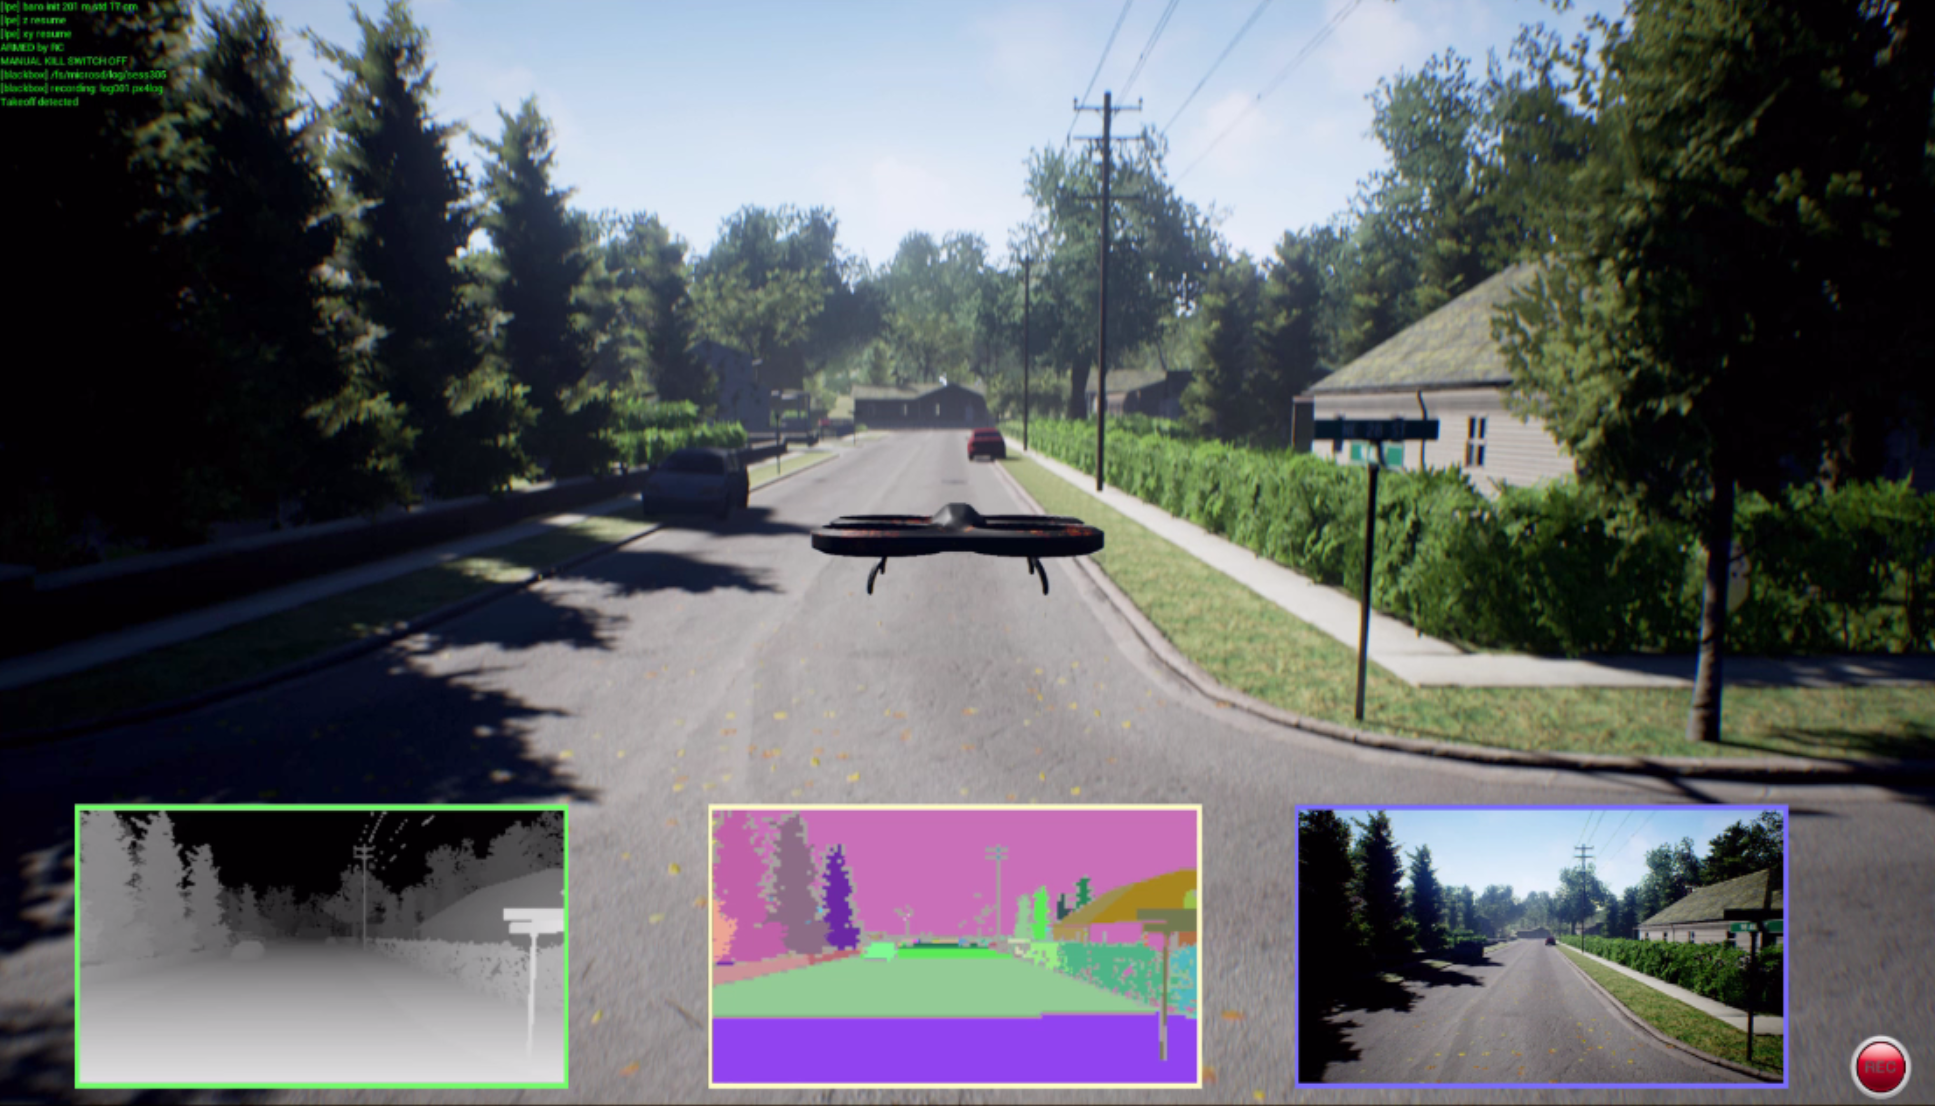
\includegraphics[width=\linewidth]{airsim.png}
    \captionof{figure}{The AirSim program}
    \label{airsim}
\end{Figure}

\subsubsection{Environments}
As has been mentioned before, the ability to use pre-built environment for the 
deployment of the drone in the simulation exists. Since the application of 
deep learning to quadcopter command has been executed before \cite{DroneRLUsingTransferLearning}, the same environments 
can be used in this thesis. These environments have been developed by the 
researchers with the goal of training the drone in a navigation task in mind. 
Examples of these environments 
can be seen in Figure \ref{env}. They contain hallways and indoor furniture 
in order to make sure that the drone can train in environments that are representative 
for the task. This pack contains a total of eleven environments, where a set of factors 
have been randomized (e.g. wallpaper pattern) for generalisability purposes. 

\begin{Figure}
    \centering
    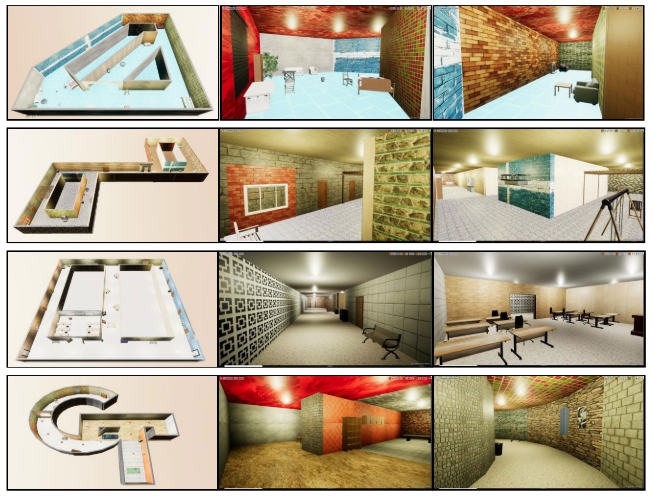
\includegraphics[width=\linewidth]{environmentstiny.png}
    \captionof{figure}{Examples of environments used during offline phase}
    \label{env}
\end{Figure}

\subsubsection{HER and State-space}
In order to measure the first research question (\ref{research1}), 
whether the addition of HER to the training process reduces the 
training time, both processes will be performed and evaluated separately. 
For the second research question (\ref{research2}), the comparison between 
normal image input and depth-image as an input for the RL is tested. This will 
happen by using the faster of the two options (HER or no HER) and performing 
training for both options will answer this question. 

\subsection{Online Phase}
Finally, the complete trained pipeline will be implemented on the ED and on 
the physical drone. In this online phase, the better performing implementation 
from the previous processes will be tested to see whether the transfer to the 
physical drone translates to similar behavior.  

\subsection{Hardware}
The devices that comprises the drone is split 
into a couple of subsections. The primary aspect is the actual quadcopter that keeps 
the device in the air and can take actions. Next to this, the device that actually 
carries the computational load of the desired autonomous behavior is attached separately. 

The drone used in this thesis is the RDDRONE-FMUK66 model, as seen in Figure \ref{Drone}.
This device is a lightweight version of a drone that needs to be assembled component 
by component making it easily modifiable. Important 
to note, is the fact that the drone comes with the availability of controlling the 
drone using a high-level API called PixHawk. This can be used to control the drone 
from different devices with commands such as "Up" and "Forward" without going into 
the details of determining how to instruct the rotors separately. This makes 
the output of the RL agent easily defined and transferred to the physical
drone.

\begin{Figure}
    \centering
    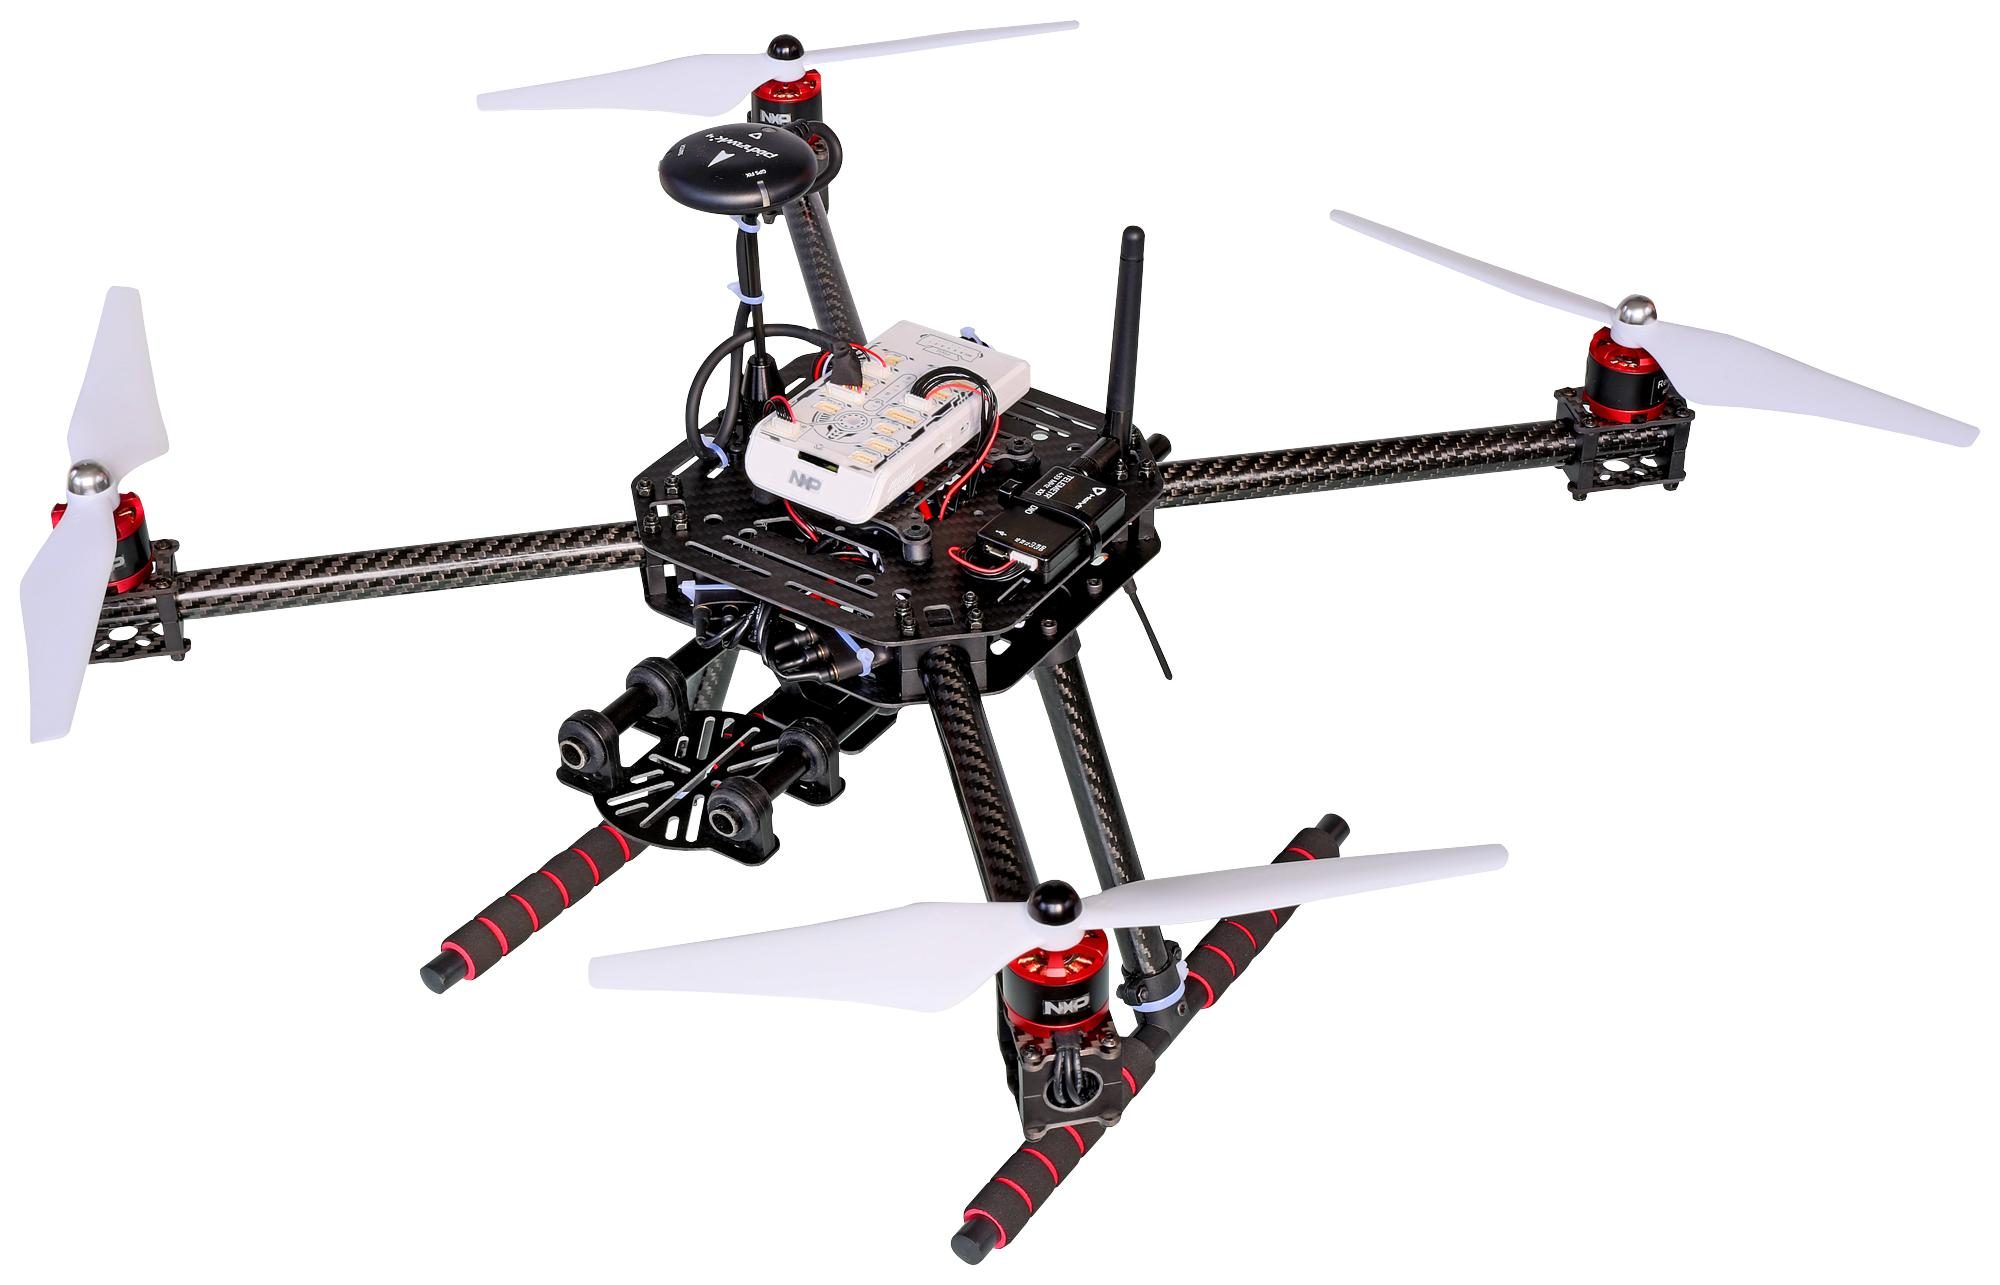
\includegraphics[width=\linewidth]{drone.jpg}
    \captionof{figure}{The RDDRONE-FMUK66 drone }
    \label{Drone}
\end{Figure}

The ED used in this thesis is the Raspberry Pi (RP) 4B 
with 4GB of RAM. The RP has the advantage of being physically small but without adding 
the problem of completely designing an embedded device for this single purpose task. 

The technology performing the depth-perception that has been chosen is a form of 
stereo vision. For the RP, there is already a starter kit that includes 
all the necessary hardware and software requirement to create a depth image. This 
kit, the StereoPi \cite{StereoPi}, includes two cameras and additional libraries to 
help with easy connection to the RP. Furthermore, the StereoPi includes a module that 
can additionally perform some computations. This helps remove some load from the 
RP so that the focus can be on performing the object detection and path planning.
The images that this camera will produce, will first be used to calculate a depth-image,
which will then be used as a potential input to the RL agent. 
